\documentclass[12pt]{article}

\usepackage{graphicx}

\begin{document}

\title{NavUP - SRS Use Case: View Traffic Congestion}
\author{SJ du Plooy (12070794)}
\date{\today}
\maketitle


\begin{tabular}{|p{4cm}|p{10cm}|}
\hline

Use Case Element & Description \\
\hline

Use Case Name & 
View Traffic Congestion \\
\hline

Use Case Description & 
The user will be able to plan ahead by viewing the current traffic congestion to a desired location, and can then decide whether he or she has time to travel to that location, or would rather go at a later stage.   \\
\hline

Primary Actor & 
Student/staff/guest \\
\hline

Precondition & 
The user must be within the campus map boundaries and have an active Wi-Fi connection.   \\
\hline

Trigger & 
When the user taps on the feature to view traffic on a given route.   \\
\hline

Basic Flow & 
When the user is on the main screen of the application, the user can:
\begin{enumerate}
\item Tap on "View Traffic Congestion"
\item Pick a destination
\item Then see the approximate congestion from the user's current location to requested destination.
\end{enumerate} \\
\hline

\hline
\end{tabular}

\begin{figure}

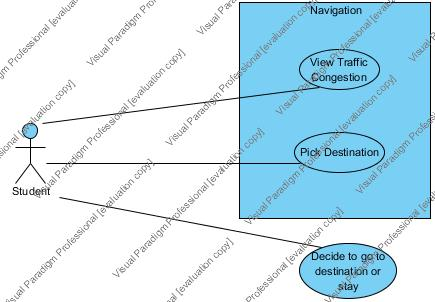
\includegraphics[width=\linewidth]{UseCaseDiagram_ViewTrafficCongestion.jpg}
\caption{Use Case Diagram of the View Traffic Congestion Use Case.}
\label{fig:UCD1}

\end{figure}

Figure \ref{fig:UCD1} View Traffic Congestion Use Case Diagram

\end{document}
